\documentclass{article}

\usepackage{amsmath}
\usepackage{amsthm}
\usepackage{amsfonts}
\usepackage{listings}
\usepackage{xcolor} 
\usepackage{graphicx}
\usepackage{subcaption}
\usepackage[utf8]{inputenc}
\usepackage[russian]{babel}

\DeclareMathOperator*{\argmax}{arg\,max}
\DeclareMathOperator*{\argmin}{arg\,min}

\DeclareMathOperator{\diag}{diag}
\DeclareMathOperator{\tr}{tr}
\DeclareMathOperator{\vect}{vec}

\newcommand{\R}{\mathbb{R}}
\newcommand{\RV}[1] {\mathbb{R}^{#1}}
\newcommand{\RM}[2] {\mathbb{R}^{#1 \times #2}}
\newcommand{\norm}[1]{\left\lVert#1\right\rVert}

\title{Домашнее задание I}
\author{Кобылянский А.В. \\ Группа 5381 \\ Вариант 2}
\date {}


\definecolor{mygreen}{RGB}{28,172,0} % color values Red, Green, Blue
\definecolor{mylilas}{RGB}{170,55,241}


\begin{document}


    \lstset{language=Octave,
        breaklines=true,
        keywordstyle=\color{blue},
        identifierstyle=\color{black},
        stringstyle=\color{mygreen},
        commentstyle=\color{gray},
        showstringspaces=false,%without this there will be a symbol in the places where there is a space
        numbers=left,%
        numberstyle={\tiny \color{black}},% size of the numbers
        numbersep=9pt, % this defines how far the numbers are from the text
        emph=[1]{for, endfor, end, break},emphstyle=[1]\color{red}, %some words to emphasise
        %emph=[2]{word1,word2}, emphstyle=[2]{style},    
    }

    \pagenumbering{gobble}
    \maketitle
    \newpage
    \pagenumbering{arabic}
         
    \subsection*{Задача 1}
    
    Запишите в эквивалентной форме каждое из следующих выражений, используя
 указанные в скобках матрицы/векторы и три      
    операции: матричное произведение,
 транспонирование и конструирование диагональной матрицы diag(𝑥).
    \bigbreak
     
    2. $ (x \in \mathbb{R}^m, y \in \mathbb{R}^n, A \in \mathbb{R}^{m \times n}), 
    \sum_{i=1}^{m} \sum_{j=1}^{n} a_{ij}x_{i}y_{j} $    
    \begin{equation*}
         \sum_{i=1}^{m} \sum_{j=1}^{n} a_{ij}x_{i}y_{j} = x^{T}Ay
    \end{equation*}
 
    4. $ (V = [v_1, ..., v_k] \in \mathbb{R}^{n \times k}, U = [u_1, ..., u_k] \in \mathbb{R}^{m \times k})\sum_{i=1}^{k} u_{i}v_{i}^{T} $    
    \begin{equation*}
         \sum_{i=1}^{k} u_{i}v_{i}^{T} = UV^T
    \end{equation*}
    
    6. $(y \in \mathbb{R}^n, A \in \mathbb{R}^{m \times n}), B := [a_{ij}y_i]_{ij}$
    \begin{equation*}
         B = A\diag(y)
    \end{equation*}
    
    8. $
    (\Sigma \in \mathbb{R}^{k \times s}, 
    V = [v_1, ..., v_s] \in \mathbb{R}^{n \times s},
    U = [u_1, ..., u_k] \in \mathbb{R}^{m \times k}), 
    \sum_{i=1}^{k} \sum_{j = 1}^{s} \Sigma_{ij}u_i v_j^T 
    $
    \begin{equation*}
        \sum_{i=1}^{k} \sum_{j = 1}^{s} \Sigma_{ij}u_i v_j^T = U\Sigma V^T
    \end{equation*}
    
    
    \subsection*{Задача 2}
    
    Пусть $ A = A^{T} \in \mathbb{R}^{n \times n}, D = D^T \in \mathbb{R}^{m \times m}$ и $ B \in \mathbb{R}^{n \times m}$
    \bigbreak
    
    2. Показать, что если $A \succ 0$ (положительно определенная матрица), то
    \begin{equation*}
         \min_{x \in \mathbb{R}^{n}} 
         \begin{bmatrix} x \\ y \end{bmatrix}^T
         \begin{bmatrix} A & B \\ B^T & D \end{bmatrix}
         \begin{bmatrix} x \\ y \end{bmatrix}
         = y^T(D-B^TA^{-1}B)y
    \end{equation*}
    
  
    $A \succ 0 \Rightarrow det(A) \neq 0$, из пункта 1 имеем:
    \begin{equation*}
         \begin{bmatrix} x \\ y \end{bmatrix}^T
         \begin{bmatrix} A & B \\ B^T & D \end{bmatrix}
         \begin{bmatrix} x \\ y \end{bmatrix}
         = (x + A^{-1}By)^{T}A(x + A^{-1}By) +
         y^T(D-B^TA^{-1}B)y
    \end{equation*}
    
    Правое слагаемое не зависит от x, необходимо минимизировать левое слагаемое.
    Выражение $z^{T}Az$ достигает минимума при $z = 0$, т.к. $A$ - положительно определена.
    При $x = -A^{-1}By$:
    \begin{equation*}
         \begin{bmatrix} x \\ y \end{bmatrix}^T
         \begin{bmatrix} A & B \\ B^T & D \end{bmatrix}
         \begin{bmatrix} x \\ y \end{bmatrix}
         = 0^{T}A0 + y^T(D-B^TA^{-1}B)y = y^T(D-B^TA^{-1}B)y
    \end{equation*}

    
    \subsection*{Задача 3}
    
    Пусть $H = H^T \in \mathbb{R}^{n \times n}$, а также $H \succ 0$. Найти
    \begin{equation*}
         \argmax_{x \in \mathbb{R}^n} \frac{x^T Hx}{x^T x}
    \end{equation*}
    
    Т.к. $H$ - симметрична, то $H = U\Lambda U^T$, где $\Lambda$ - диагональная матрица собственных значений, $U^{-1} = U^T$. Все элементы $\Lambda$ действительны и положительны, т.к. $H \succ 0$. Пусть $y = U^Tx$
    \begin{align*}
         \frac{x^T Hx}{x^T x} &= \frac{y^TU^T U\Lambda U^TUy}{y^TU^TUy} = \frac{y^T\Lambda y}{y^Ty} = \frac{\sum_i \lambda_i y_i^2}{\sum_i y_i^2}\\
         \frac{\partial f}{\partial y_i} &= \frac{2y_i\lambda_i\sum_i y_i^2 - 2y_i\sum_i \lambda_i y_i^2}{(\sum_i y_i^2)^2} = 0 \Rightarrow 
         \left[ 
            \begin{gathered}
                y_i = 0 \\ 
                \lambda_i = \frac{\sum_i \lambda_i y_i^2}{\sum_i y_i^2}
            \end{gathered} 
        \right.
    \end{align*}
    
    
    
    Пусть $U$ выбрана так, чтобы собственные числа в $\Lambda = \diag([\lambda_1, ..., \lambda_n])$ шли по невозрастанию $\lambda_1 \geq \lambda_2 \geq ... \geq \lambda_n$. 
    
    $y$ будет стационарной точкой, если $f(y) = \lambda_i$ и $\forall j: \lambda_j \neq \lambda_i \Rightarrow y_j = 0$, следовательно $\max f(y) = \lambda_1$. Пусть первые $k$ собственных чисел одинаковы, т.е. $\lambda_1 = ... = \lambda_k \neq \lambda_{k+1}$, тогда максимум достигается для $y = [y_1, ..., y_k, 0, ..., 0]$, где $y_1, ..., y_k$ - принимают любые значения, кроме всех нулей, т.е. $y \neq 0$. $Uy$ - линейная комбинация собственных векторов, соответствующих собственному числу $\lambda_1$ 
    
    Ответ: функция достигает максимума на $x$ из собственного подпространства максимальнго собственного числа матрицы $H$, $x \neq 0$.
    \newpage
    
    \subsection*{Задача 4}
    Для каждой из следующих функций $f(x)$ выписать первый дифференциал. Для
 скалярных функций векторного аргумента найти вектор-градиент $\nabla f(x)$ и матрицу Гессе $\nabla^2 f(x)$.
 Для скалярных функций матричного аргумента найти матрицу-градиент $\nabla f(X)$. Для векторных
 функций векторного аргумента найти матрицу Якоби $J(x)$.
    
    Для каждого пункта сделать численную проверку градиента.
    \bigbreak
    
    Функция для численной проверки градиента.
    \lstinputlisting{Octave/grad_check.m}
    \bigbreak
    
    2. $f(x) = \exp(A\exp(B\exp(Cx)))$, где $\exp(y) = [e^{y_1}, ..., e^{y_n}]^T, x \in \mathbb{R}^n$
    \bigbreak
    Посчитав частные производные $\exp(x)$ легко видеть, что матрица Якоби для этой функции равна $\diag(\exp(x))$, следовательно $d\exp(x) = \diag(\exp(x))dx$.    
    \begin{align*}
        &d\exp(A\exp(B\exp(Cx))) = \diag(\exp(A\exp(B\exp(Cx))))Ad\exp(B\exp(Cx)))=\\
        &= \diag(\exp(A\exp(B\exp(Cx))))A\diag(\exp(B\exp(Cx))))Bd\exp(Cx)) = \\
        &= \diag(\exp(A\exp(B\exp(Cx))))A\diag(\exp(B\exp(Cx)))B\diag(\exp(Cx))Cdx
    \end{align*}
    
    Матрица Якоби $J(x)$
    \begin{equation*}
         J(x) = \diag(\exp(A\exp(B\exp(Cx))))A\diag(\exp(B\exp(Cx)))B\diag(\exp(Cx))C
    \end{equation*}
    
    Численная проверка
    \lstinputlisting[firstline=3, lastline=16]{Octave/checks.m}
    \bigbreak
    
    4. $f(X) = \tr(AX^{-1}B), X \in \mathbb{R}^{n \times n}$
    \begin{align*}
        &d\tr(AX^{-1}B) = \tr(d(AX^{-1}B)) = \tr(Ad(X^{-1})B) =\\
        = &\tr(-AX^{-1}dXX^{-1}B) = \tr(-X^{-1}BAX^{-1}dx) =\\
        = &\tr(-(X^{-T}A^TB^TX^{-T})^Tdx)
    \end{align*}
    
    Матрица градиент $\nabla f(x)$
    \begin{equation*}
         \nabla f(x) = -X^{-T}A^TB^TX^{-T}
    \end{equation*}
    
    Численная проверка
    \lstinputlisting[firstline=19, lastline=30]{Octave/checks.m}
    \newpage
    
    6. $f(X) = \tr\left(\left[
                \begin{matrix}
                X & B\\
                B^T & A
                \end{matrix}
                \right]\right), X \in \mathbb{R}^{n \times n}$
    \begin{align*}
        d\tr\left(\left[
                \begin{matrix}
                X & B\\
                B^T & A
                \end{matrix}
                \right]\right) = d(\tr(X) + \tr(A)) = \tr(dX)
    \end{align*}
    
    Матрица градиент $\nabla f(x)$
    \begin{equation*}
         \nabla f(x) = I
    \end{equation*}
    
    Численная проверка
    \lstinputlisting[firstline=34, lastline=45]{Octave/checks.m}
    \bigbreak
    
    8. $f(X) = \det(X^TAX), X \in  \RM{n}{n}$
    \begin{align*}
        &d\det(X^TAX) = \det(X^TAX)\tr((X^TAX)^{-1}d(X^TAX)) =\\
        = &\det(X)^2\det(A)\tr((X^TAX)^{-1}(dX^TAX + X^TAdX)) =\\ 
        = &\det(X)^2\det(A)(\tr(X^{-1}A^{-1}X^{-T}dX^TAX) + \tr(X^{-1}A^{-1}X^{-T}X^TAdX))\\
        = &\det(X)^2\det(A)tr(2X^{-1}dX)
    \end{align*}
    
    Матрица градиент $\nabla f(x)$
    \begin{equation*}
         \nabla f(x) = 2\det(X)^2\det(A)X^{-T}
    \end{equation*}
    
    Численная проверка
    \lstinputlisting[firstline=48, lastline=58]{Octave/checks.m}
    \bigbreak
    
    10. $f(X) = \log\det(X^p), X \in  \RM{n}{n}$
    \begin{align*}
        d\log\det(X^p) &= d(\log\det(X)^p) = d(p\log\det(X)) =\\
        = p\frac{d\det(X)}{\det(X)} &= p\frac{\det(X)\tr(X^{-1}dX)}{\det(X)} = p\tr(X^{-1}dX)
    \end{align*}
    
    Матрица градиент $\nabla f(x)$
    \begin{equation*}
         \nabla f(x) = pX^{-T}
    \end{equation*}
    
    Численная проверка
    \lstinputlisting[firstline=62, lastline=72]{Octave/checks.m}
    \bigbreak
    
    12. $f(X) = \frac{1}{2}\norm{AX - B}^2_F, x \in \RM{m}{n}$
    \begin{align*}
        d\frac{1}{2}\norm{X}^2_F &= \frac{1}{2}d((\tr(X^TX)^{0.5})^2) = \frac{1}{2}\tr(d(X^TX)) =
        \frac{1}{2}\tr(dX^TX + X^TdX) = \tr(X^TdX)\\
        d\frac{1}{2}\norm{AX - B}^2_F &= \tr((AX - B)^TAdX)
    \end{align*}
    
    Матрица градиент $\nabla f(x)$
    \begin{equation*}
         \nabla f(x) = A^T(AX - B)
    \end{equation*}
    
    Численная проверка
    \lstinputlisting[firstline=76, lastline=87]{Octave/checks.m}
    \bigbreak
    
    14. $f(X) = \log(\sum_{i = 1}^{n} \exp(a_i^Tx)), x \in \RV{n}$
    \bigbreak
    
    Пусть $A = [a_1, ..., a_n]$ - матрица из столбцов $a_i$, $1 = [1, ..., 1]^T \in \RV{n}$, тогда
    \begin{align*}
        \log(\sum_{i = 1}^{n} \exp(a_i^Tx)) &= \log( 1^T\exp(A^Tx))\\
        d\log( 1^T\exp(A^Tx)) &= \frac{1^Td\exp(A^Tx)}{1^T\exp(A^Tx)} = 
        \frac{1^T\diag(\exp(A^Tx))A^Tdx}{1^T\exp(A^Tx)} =
        \frac{\exp(A^Tx)^TA^Tdx}{1^T\exp(A^Tx)}
    \end{align*}
    
    Вектор градиент $\nabla f(x)$
    \begin{equation*}
         \nabla f(x) = \frac{A\exp(A^Tx)}{1^T\exp(A^Tx)}
    \end{equation*}
    
    Найдем вторую производную
    \begin{align*}
        &d\left(\frac{\exp(A^Tx)^TA^Tdx_1}{1^T\exp(A^Tx)}\right) =
        \frac{d(\exp(A^Tx)^TA^Tdx_1)1^T\exp(A^Tx) - \exp(A^Tx)^TA^Tdx_1d(1^T\exp(A^Tx))}{(1^T\exp(A^Tx))^2} =\\
        = &\frac{dx_2^TA\diag(\exp(A^Tx))A^Tdx_11^Texp(A^Tx) -
        \exp(A^Tx)^TA^Tdx_11^T\diag(\exp(A^Tx))A^Tdx_2}{(1^T\exp(A^Tx))^2)} =\\
        = & | v := \exp(A^Tx) | = 
        \frac{((dx_1)^TA\diag(v)A^Tdx_2)1^Tv - (dx_1)^TAvv^TA^Tdx_2}{(1^Tv)^2} =\\
        = &\frac{ (dx_1)^TA(1^Tv\diag(v) - vv^T)A^Tdx_2}{(1^Tv)^2}
    \end{align*}
    
    Матрица Гессе $\nabla^2 f(x)$
    \begin{equation*}
         \nabla^2 f(x) = \frac{ A(1^Tv\diag(v) - vv^T)A^T}{(1^Tv)^2}, \text{где } v = \exp(A^Tx)
    \end{equation*}
    
    
    Численная проверка
    \lstinputlisting[firstline=91, lastline=105]{Octave/checks.m}
    \bigbreak
    
    16. $f(X) = \tr((X^TCX)^{-1}A), X \in \RM{n}{n}, A, C$ - симметричные матрицы
    \begin{align*}
        &d\tr((X^TCX)^{-1}A) = \tr(d(X^{-1}C^{-1}X^{-T}A)) =\\ 
        = &\tr(dX^{-1}C^{-1}X^{-T}A + X^{-1}C^{-1}dX^{-T}A) =\\
        = &\tr(C^{-1}X^{-T}AdX^{-1} + AdX^{-1}C^{-1}X^{-T}) =\\ 
        = &\tr(2C^{-1}X^{-T}AdX^{-1}) =\\
        = &-2\tr(C^{-1}X^{-T}AX^{-1}dXX^{-1}) =\\
        = &-2\tr(X^{-1}C^{-1}X^{-T}AX^{-1}dX) =\\
        = &-2\tr((X^TCX)^{-1}AX^{-1}dX)
    \end{align*}
    
    Матрица градиент $\nabla f(x)$
    \begin{equation*}
         \nabla f(x) = X^{-T}A^TX^{-1}C^{-T}X^{-T}
    \end{equation*}
    
    Численная проверка
    \lstinputlisting[firstline=109, lastline=120]{Octave/checks.m}
    \newpage
    
    \subsection*{Задача 5}
    Для каждой из следующих функций найти все стационарные точки и определить их
 тип (локальный максимум/минимум, седловая точка).
    \bigbreak
    
    2. $f(x) = (1- x_1)^2 + 100(x_2 - x_1)^2$
    
    \begin{align*}
        \nabla f(x) &= 
                \left[
                \begin{matrix} 
                    \frac{\partial f}{\partial x_1}\\
                    \frac{\partial f}{\partial x_2}
                \end{matrix}
                \right] 
                = 
                \left[
                \begin{matrix} 
                    202x_1 - 200x_2 - 2\\
                    -200_1 + 200x_2
                \end{matrix}
                \right]\\
        \nabla f(x) &= 0 \Rightarrow x_1 = 1, x_2 = 1
    \end{align*}
    
    $f(x)$ имеет единственную стационарную точку $x = [1, 1]$. Очевидно, что это точка глобального минимума. Убедимся в этом, рассмотря $\nabla^2 f(x)$
    
    \begin{align*}
        \nabla^2 f(x) = 
                \left[
                \begin{matrix} 
                    \frac{\partial^2 f}{\partial x_1^2} &
                    \frac{\partial^2 f}{\partial x_1 \partial x_2}\\                    
                    \frac{\partial^2 f}{\partial x_1 \partial x_2} &
                    \frac{\partial^2 f}{\partial x_1}
                \end{matrix}
                \right] 
                = 
                \left[
                \begin{matrix} 
                    202 & -200\\
                    -200 & 200
                \end{matrix}
                \right]\\
    \end{align*}
    
    Собственные числа $\nabla^2 f(x)$ равны $\lambda_{1,2} = 201 \pm \sqrt{40001} > 0$. Оба числа положительны, значит $\nabla^2 f(x) \succ 0$ и $x = [1, 1]$ - точка строгого глобального минимума.
    \bigbreak
    
    4. $f(x) = \vect(xa^T)^T\vect(xb^T)$
    \begin{align*}
        \vect(xa^T)^T\vect(xb^T) &= \tr((xa^T)^Txb^T) =\\
        = \tr(ax^Txb^T) &= \tr(a^Tbx^Tx) = a^Tbx^Tx\\
        d(a^Tbx^Tx) &= 2a^Tbx^Tdx\\
        \nabla f(x) &= 2a^Tbx = 0 \Rightarrow x = 0 \vee a^Tb = 0\\ 
        \nabla^2 f(x) &= 2a^TbI_n
    \end{align*}
        
    При $ a^Tb \neq 0$  $f(x)$ имеет единственную стационарную точку $x = 0$. При $a^Tb > 0$ это точка глобального минимума, при $a^Tb < 0$ это точка глобального максимума. 
    
    При $a^Tb = 0 $ $f(x) \equiv 0$ и все точки $\RV{n}$ будут точками точками минимума и максимума одновременно.
    \newpage
    
    \subsection*{Задача 6}
    Для каждой задачи оптимизации найти множество решений и оптимальное значение
 целевой функции.
    \bigbreak
    
    2. $\min\limits_{x \in \RV{n}} x^TAx - x^Tb, A \succ 0$
    \begin{align*}
       d(x^TAx - x^Tb) &= 2x^TAdx - dx^Tb = (2x^TA - b^T)dx =\\
       \nabla f(x) &= 2Ax - b = 0 \Rightarrow x^* = 0.5A^{-1}b\\
       d((2x^TA - b^T)dx_1) &= (dx_1)^T2Adx_2\\
       \nabla^2 f(x) &= 2A \succ 0
    \end{align*}
    
    Так как $\nabla^2 f(x) \succ 0$, то функция выпукла и любая стационарная точка будет глобальным минимумом, значи $x^*$ - точка глобального минимума.
    \begin{align*}
       f(x^*) &= (\frac{1}{2}A^{-1}b)^TA(\frac{1}{2}A^{-1}b) - (\frac{1}{2}A^{-1}b)^Tb =\\
       &=\frac{1}{4}b^TA^{-1}b - \frac{1}{2}b^TA^{-1}b = -\frac{1}{2}b^TA^{-1}b
    \end{align*}
    
    Ответ: $x^* = \frac{1}{2}A^{-1}b, f(x^*) = -\frac{1}{2}b^TA^{-1}b$
    \bigbreak
    
    4. $\min\limits_{x \in \RV{n}} c^Tx + \frac{\alpha}{3}\norm{x}^3, \alpha > 0$
    \begin{align*}
       d \frac{1}{3}\norm{x}^3 &= \frac{1}{3}d(x^Tx)^{\frac{3}{2}} = 
       \frac{1}{3}\frac{3}{2}(x^Tx)^{\frac{1}{2}}d(x^Tx) =
       \frac{1}{2}\norm{x}(2x^Tdx) = \norm{x}x^Tdx\\
       d(c^Tx + \frac{\alpha}{3}\norm{x}^3) &= (c^T + \alpha\norm{x}x^T)dx\\
       \nabla f(x) &= c + \alpha\norm{x}x = 0 \Rightarrow \norm{(\alpha\norm{x}x)} = \norm{-c} \Rightarrow \norm{x} = \sqrt{\frac{\norm{c}}{a}} \Rightarrow
       x^* = -\frac{c}{\sqrt{\alpha\norm{c}}}
    \end{align*}
    
    Найдем $\nabla^2 f(x)$    
    \begin{align*}
       d((c^T + \alpha\norm{x}x^T)dx_1) &=
       \alpha(d(\norm{x})x^Tdx_1 + \norm{x}d(x^Tdx_1)) =\\
       &= \alpha((\frac{1}{2}(x^Tx)^{-\frac{1}{2}}(2x^Tdx_2))(x^Tdx_1) 
       \norm{x}((dx_2)^Tdx_1)) =\\
       &=\alpha(\norm{x}^{-1}(x^Tdx_2)(x^Tdx_1) + \norm{x}(dx_2^Tdx_1)) =\\
       &= (dx_1)^T\alpha(\norm{x}^{-1}xx^T + \norm{x}I_n)dx_2\\
       \nabla^2 f(x) &= \alpha(\norm{x}^{-1}xx^T + \norm{x}I_n) =
       \alpha\norm{x}\left(\frac{xx^T}{\norm{x}^2} + I_n\right)
    \end{align*}
    
    Пусть $ x \neq 0$. $\frac{xx^T}{\norm{x}^2}$ - одноранговая матрица у которой все собственные числа равны 0, кроме одного, соответствующего собственному вектору $x$, равного 1.
    \begin{align*}
        \left( \frac{xx^T}{\norm{x}^2}\right)x =
        \frac{x(x^Tx)}{\norm{x}^2} =
        \frac{x\norm{x}^2}{\norm{x}^2} = x        
    \end{align*}
    
    Собственные числа $xx^T/\norm{x}^2 + I_n$ равны соответственно 1 и 2. Т.к. все собственные числа положительны, матрица положительно определена, $\alpha\norm{x} > 0$, значит $\nabla^2 f(x) \succ 0$.
    
    Пусть $x = 0$. $\nabla^2 f(0) = 0$, значит
    \begin{align*}
        \forall x \in \RV{n} \: \nabla^2 f(x) \succeq 0 \Rightarrow f(x) - \text{выпукла } \Rightarrow x^* - \text{глобальный минимум}\\
        \\
        f(x^*) = -\frac{c^Tc}{\sqrt{\alpha\norm{c}}} +
        \frac{\alpha}{3}\frac{\norm{c}^3}{(\alpha\norm{c})^{\frac{3}{2}}} =
        -\frac{\norm{c}^{\frac{3}{2}}}{\sqrt{\alpha}} +
        \frac{1}{3}\frac{\norm{c}^{\frac{3}{2}}}{\sqrt{\alpha}} =
        -\frac{2}{3}\frac{\norm{c}^{\frac{3}{2}}}{\sqrt{\alpha}}
    \end{align*}
    
    Ответ: $x^* = -\frac{c}{\sqrt{\alpha\norm{c}}}, f(x^*) = -\frac{2}{3}\frac{\norm{c}^{\frac{3}{2}}}{\sqrt{\alpha}}$
    \bigbreak
    
    6.  $\min\limits_{x \in \RV{n}_+, 1^Tx = 1} a^Tx, a \in \RV{n}_+$
    
    Сумма компонент $x_i$ должна быть равна 1. Чтобы значение функции было минимально, необходимо найти минимальную из компонент $a_i$ и уствновить $x_i = 1, x_j = 0 \: j \neq i$. Если минимальны $a_i$ несколько, то обозначим
    \begin{align*}
        I_{min} = \{i \mid \forall a_j \in a : a_i \leq a_j\}
    \end{align*}
    индексы минимальных компонент $a$, тогда     
    \begin{align*}
        \argmin\limits_{x \in \RV{n}_+, 1^Tx = 1} a^Tx =
        \left\{x \in \RV{n}_+ \mid V \subset I_{min} \land \sum_{i \in V} x_i = 1 \land \forall i \notin V : x_i = 0 \right\}
    \end{align*}
    
    Минимальное значение функции равно минимальной компоненте $a$
    \begin{align*}
        \min\limits_{x \in \RV{n}_+, 1^Tx = 1} a^Tx = \min a
    \end{align*}
    \newpage
    
    \subsection*{Задача 7}
    Для данного набора переменных $u \in \RV{n}, v \in \RV{m}, z \in \mathbb{R}$ и набора констант $B \in \RM{k}{n}, C \in \RM{k}{m}, a \in \RV{k}, c \in \RV{m}$ записать систему уравнений
    \begin{equation*}
        Bu + Cv = a, v_i + z = c_i, \sum_i u_i = z
    \end{equation*}
    в виде $Ax = b$, если обозначить $x = [u; v; z] \in \RV{n + m + 1}$. То есть выразить $A$ и $b$ через $B, C, a, c$.
    \bigbreak
    
    Пусть $0_v = [0, ..., 0]^T, 1_v = [1, ..., 1]^T, I_n$ - единичная матриц, $0_m$ - матрица полностью из нулей, тогда
    \begin{align*}
    A = \left[\begin{matrix}
            B & C & 0_v \\
            0_m & I_n & 1_v \\
            1_v^T & 0_v^T & -1
        \end{matrix}\right], \:
    b = \left[\begin{matrix}
            a \\
            c \\
            0
        \end{matrix}\right]
    \end{align*}
    
    \subsection*{Задача 8}
    Рассмотрим задачу предсказания оценок пользователей для некоторых объектов,
 например, фильмов. В этом случае данные представлены матрицей размера $N\times M$, где $N$ –
 количество фильмов в базе данных, $M$ – количество зарегистрированных пользователей. Часть элементов этой матрицы известны, а значения остальных требуется предсказать.
    
    Целевая функция для настройки параметров имеет вид
    \begin{align*}
        f(P, Q) = \frac{1}{2}\sum_{n, m: r_{n, m} \neq 0} (r_{n, m} - p_n^Tq_m)^2 +
        \frac{\lambda_p}{2}\norm{P}_F^2 + \frac{\lambda_q}{2}\norm{Q}_F^2 
    \end{align*}
    
    Использовать часть оценок $(R)$ для нахождения оптимальных параметров $(P^*, Q^*) =
 \argmin_{P, Q} f(P, Q)$ с помощью ALS. Реализовать ALS. Использовать $K = 10 - 15$ и $\lambda_p = \lambda_q = \lambda$, где
 $\lambda = \{0.001, 0.01, 0.1\}$. Построить графики зависимости целевой функции от номера итерации для
нескольких значений $\lambda$. Построить графики зависимости среднеквадратичной ошибки (root-meansquare error, RMSE) для тестовой (R test) и обучающей (R) выборок от номера итерации для нескольких значений $\lambda$.   
    \newpage
    
    Функция, реализующая ALS
    \lstinputlisting{Octave/als.m}
    \bigbreak
     
    Функция, расчитывающая $f(P, Q)$ и RMSE
    \lstinputlisting{Octave/tests.m}     
    
    \begin{figure}[h!]
        \centering
        \begin{subfigure}[b]{0.4\linewidth}
            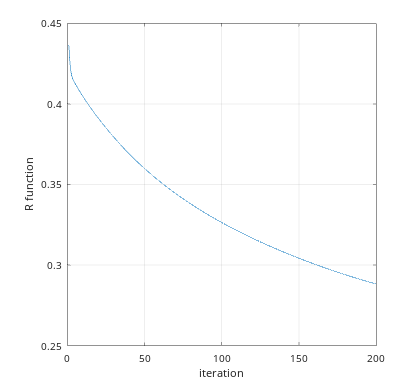
\includegraphics[width=\linewidth]{Plots/R_fun_0_001.png}
            \caption{$\lambda = 0.001$}
        \end{subfigure}
        \begin{subfigure}[b]{0.4\linewidth}
            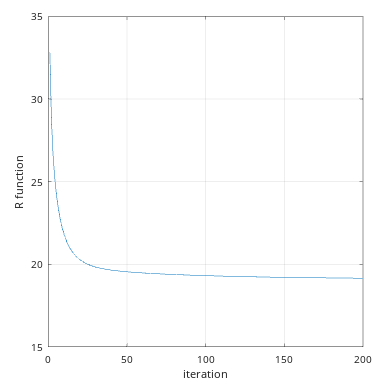
\includegraphics[width=\linewidth]{Plots/R_fun_0_1.png}
            \caption{$\lambda = 0.1$}
        \end{subfigure}
        \caption{Графики зависимости целевой функции от итерации}
    \end{figure}
    
    \begin{figure}
        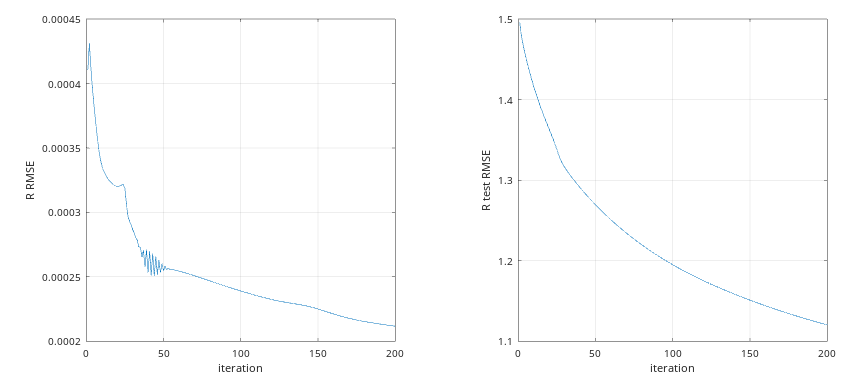
\includegraphics[width=\linewidth]{Plots/RMSE_0_001.png}
        \caption{Графики зависимости RMSE для R и R\textunderscore test от итерации при $\lambda = 0.001$}
    \end{figure}
    
    \begin{figure}
        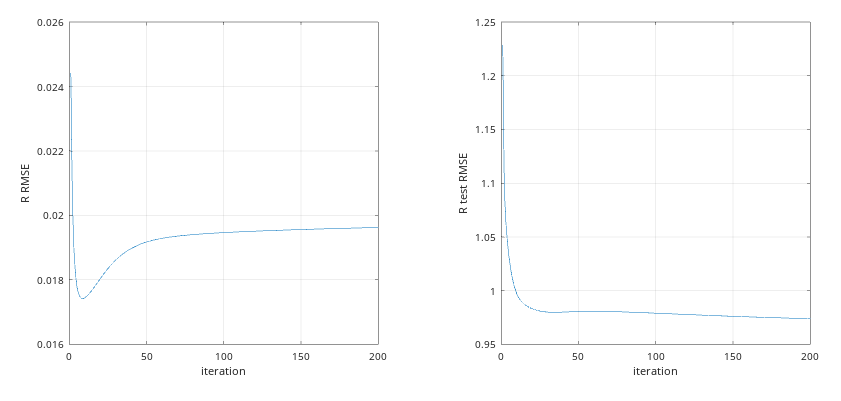
\includegraphics[width=\linewidth]{Plots/RMSE_0_1.png}
        \caption{Графики зависимости RMSE для R и R\textunderscore test от итерации при $\lambda = 0.1$}
    \end{figure}
\end{document}

    


    
    
